\chapter{Resultados}
En este capítulo se recogen los resultados obtenidos con las versiones finales del código, que son las que se entregan junto a esta memoria. Todos los tiempos mostrados en este capítulo han sido calculados con el cálculo de la media tras diez repeticiones, y en el caso de CUDA se ha tomado el valor del TPB que ofrecía mejores tiempos.

En la Tabla \ref{TiemposPC} se muestran los resultados obtenidos con el equipo con prestaciones más limitadas. Se llega a obtener una aceleración máxima de 4.89x en la versión con OpenACC para 4 dimensiones. Para CUDA, la aceleración máxima es de 24.44x para la versión bidimensional, aunque tan solo de 9.82x para la versión CUDA. La versión que utiliza la tarjeta gráfica supera, como se esperaba, a la versión paralelizada con CPU, pero estas aceleraciones se ven limitadas por las prestaciones de la tarjeta gráfica.

\begin{table}[H]
    \centering
    \begin{tabular}{llllllll}
    \multicolumn{1}{c}{} & \multicolumn{1}{c}{Secuencial} & \multicolumn{1}{c}{} & \multicolumn{2}{c}{OpenACC}        & \multicolumn{1}{c}{} & \multicolumn{2}{c}{CUDA}            \\ 
    \cline{2-2}\cline{4-5}\cline{7-8}
                         & Min. Time                      &                      & Min. Time   & Max. Speedup         &                      & Min. Time   & Max. Speedup          \\
    $128^2$                & 0.000129244                    &                      & 0.000131645 & 0.981761556          &                      & 0.000215194 & 0.600592953           \\
    $1024^2$                & 0.0082662                      &                      & 0.00264092  & 3.13004559           &                      & 0.000661026 & 12.5051057            \\
    $4096^2$                & 0.134949                       &                      & 0.0328057   & 4.11358392           &                      & 0.0059252   & 22.77543374           \\
    $8192^2$                & 0.554647                       &                      & 0.128613    & \textbf{4.312526727} &                      & 0.0226875   & \textbf{24.44725069}  \\
    $16384^2$                & 1.80975                        &                      & 0.419469    & 4.314383184          &                      & 0.0940518   & 19.24205597           \\
                    &                                &                      &             &                      &                      &             &                       \\
    $64^3$                & 0.0025754                      &                      & 0.000715507 & 3.599405736          &                      & 0,000482099  & 5.3420563             \\
    $128^3$                & 0.0204921                      &                      & 0.00421121  & \textbf{4.86608362}  &                      & 0,00411259  & 4.982772413           \\
    $256^3$                & 0.165632                       &                      & 0.0343316   & 4.824476576          &                      & 0,0276551 & 5.989202715           \\
    $512^3$                & 1.31866                        &                      & 0.273366    & 4.823789352          &                      & 0,194417  & \textbf{6.782637321}  \\
                    &                                &                      &             &                      &                      &             &                       \\
    $32^4$                & 0.012464                       &                      & 0.00254871  & \textbf{4.890317062} &                      & 0.00126846  & \textbf{9.826088328}  \\
    $64^4$                & 0.195305                       &                      & 0.0411499   & 4.746184073          &                      & 0.0278342   & 7.016727623           \\
    $128^4$                & 3.11248                        &                      & 0.701806    & 4.434957809          &                      & 0.688997    & 4.517407188          
    \end{tabular}
    \caption{Tiempos (en segundos) y aceleraciones obtenidas en PC}
    \label{TiemposPC}
    \end{table}
\raggedbottom 
En las figuras \ref{GraficoPC2D}, \ref{GraficoPC3D} y \ref{GraficoPC4D} se ven representados gráficamente los datos de la Tabla \ref{TiemposPC}.

\begin{figure}[H]
    \centering
    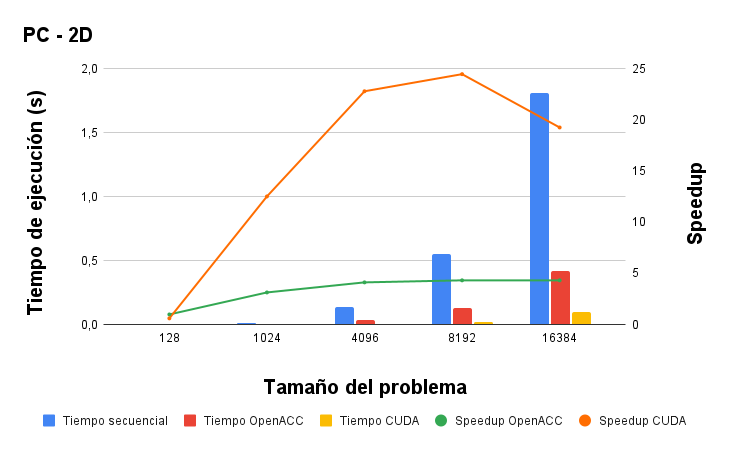
\includegraphics[width=\textwidth]{img/PC - 2D.png}
    \label{GraficoPC2D}
    \caption{Representación gráfica de los tiempos de ejecución y de las aceleraciones obtenidas en el PC para la versión 2D }
\end{figure}


\begin{figure}[H]
    \centering
    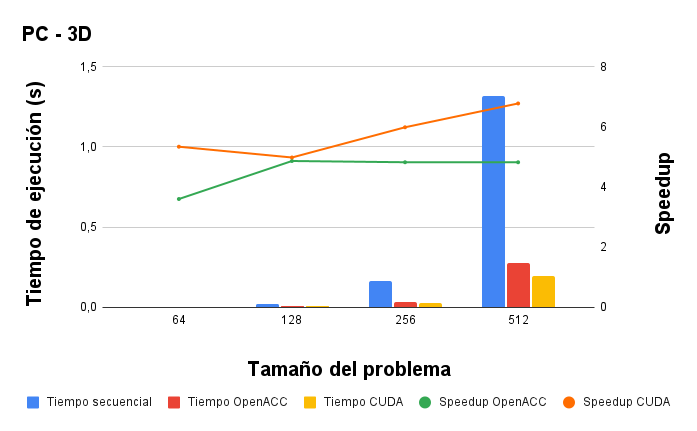
\includegraphics[width=\textwidth]{img/PC - 3D.png}
    \label{GraficoPC3D}
    \caption{Representación gráfica de los tiempos de ejecución y de las aceleraciones obtenidas en el PC para la versión 3D }
\end{figure}


\begin{figure}[H]
    \centering
    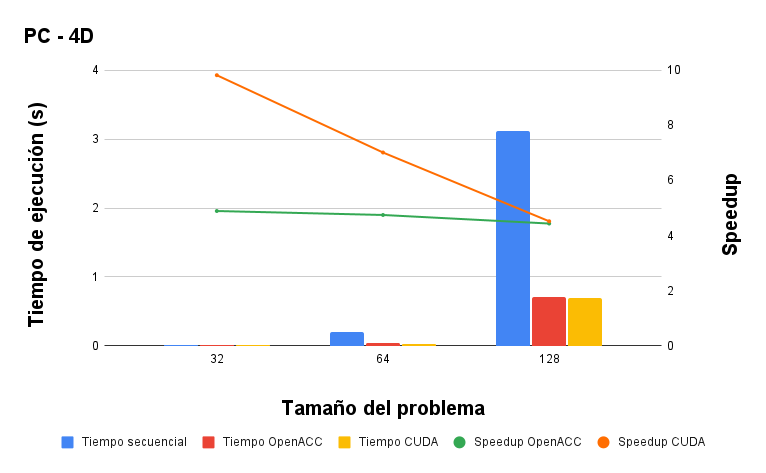
\includegraphics[width=\textwidth]{img/PC - 4D.png}
    \caption{Representación gráfica de los tiempos de ejecución y de las aceleraciones obtenidas en el PC para la versión 4D }
    \label{GraficoPC4D}
\end{figure}

Por otro lado, en la Tabla \ref{TiemposServidor} están los tiempos y aceleración obtenidas en el servidor. Además de los tamaños calculados en el primer equipo, el aumento de RAM y de memoria de la tarjeta gráfica del servidor permite la medida de tiempos para algunos tamaños superiores. La aceleración máxima obtenida para la versión con paralelismo a nivel de CPU es de 20.49x en la versión tridimensional mientras que para la versión CUDA se obtiene una aceleración máxima de 77.47x en la versión 4D.

\begin{table}[H]
    \centering
    \begin{tabular}{llllllll}
    \multicolumn{1}{c}{} & \multicolumn{1}{c}{Secuencial} & \multicolumn{1}{c}{} & \multicolumn{2}{c}{OpenACC} & \multicolumn{1}{c}{} & \multicolumn{2}{c}{CUDA}      \\ 
    \cline{2-2}\cline{4-5}\cline{7-8}
                         & Min. Time                      &                      & Min. Time & Max. Speedup    &                      & Min. Time   & Max. Speedup    \\
    $128^2$                & 0.00048                        &                      & 0.00741   & 0.06            &                      & 0.000172544 & 2.76            \\
    $1024^2$                & 0.01075                        &                      & 0.00303   & 3.55            &                      & 0.000374784 & 28.69           \\
    $4096^2$                & 0.15189                        &                      & 0.02203   & 6.89            &                      & 0.00271309  & 55.99           \\
    $8192^2$                & 0.60966                        &                      & 0.04978   & 12.25           &                      & 0.0102789   & \textbf{59.31}  \\
    $16384^2$                & 2.44145                        &                      & 0.15529   & 15.72           &                      & 0.0450243   & 54.23           \\
    $32768^2$                & 9.77276                        &                      & 0.57479   & \textbf{17}     &                      & 0.180257    & 54.22           \\
                         &                                &                      &           &                 &                      &             &                 \\
    $64^3$                 & 0.00282                        &                      & 0.0008    & 3.51            &                      & 0.00021555  & 13.07           \\
    $128^3$                 & 0.02266                        &                      & 0.00388   & 5.83            &                      & 0.00058726  & 38.58           \\
    $256^3$                 & 0.18025                        &                      & 0.02398   & 7.52            &                      & 0.00312218  & \textbf{57.73}  \\
    $512^3$                 & 1.44507                        &                      & 0.08371   & 17.26           &                      & 0.02524210  & 57.25           \\
    $1024^3$                 & 11.5543                        &                      & 0.56389   & \textbf{20.49}  &                      & 0.23780300  & 48.59           \\
                         &                                &                      &           &                 &                      &             &                 \\
    $32^4$                  & 0.01402                        &                      & 0.00266   & 5.26            &                      & 0.00032358  & 43.32           \\
    $64^4$                  & 0.22078                        &                      & 0.02091   & 10.56           &                      & 0.00284979  & \textbf{77.47}  \\
    $128^4$                  & 3.5307                         &                      & 0.21618   & \textbf{16.33}  &                      & 0.0523832   & 67.4            \\
                         &                                &                      &           &                 &                      &             &                 \\
                         &                                &                      &           &                 &                      &             &                
    \end{tabular}
    \caption{Tiempos (en segundos) y aceleraciones obtenidas en el servidor}
    \label{TiemposServidor}
    \end{table}

En las figuras \ref{GraficoServidor2D}, \ref{GraficoServidor3D}} y \ref{GraficoServidor4D} se ven representados gráficamente los datos de la Tabla \ref{TiemposServidor}.

\begin{figure}[H]
    \centering
    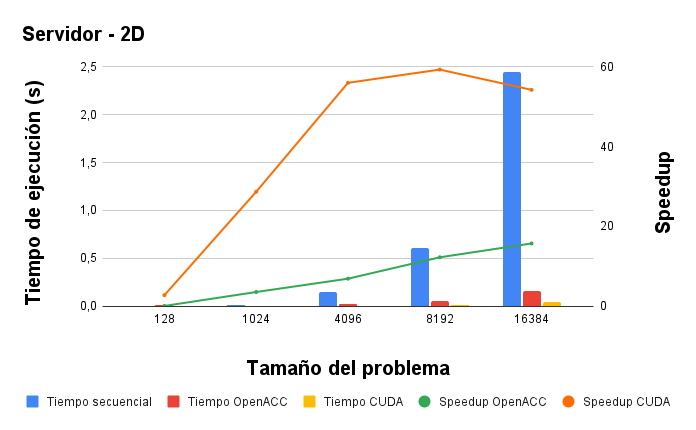
\includegraphics[width=\textwidth]{img/Servidor - 2D.png}
    \caption{Representación gráfica de los tiempos de ejecución y de las aceleraciones obtenidas en el Servidor para la versión 2D }
    \label{GraficoServidor2D}
\end{figure}

\begin{figure}[H]
    \centering
    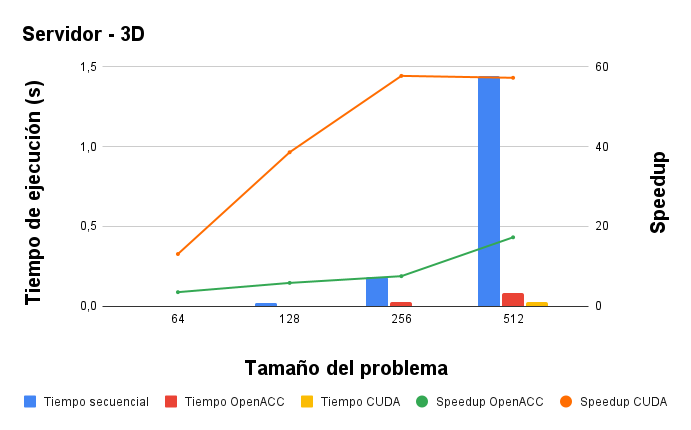
\includegraphics[width=\textwidth]{img/Servidor - 3D.png}
    \caption{Representación gráfica de los tiempos de ejecución y de las aceleraciones obtenidas en el Servidor para la versión 3D }
    \label{GraficoServidor3D}
\end{figure}

\begin{figure}[H]
    \centering
    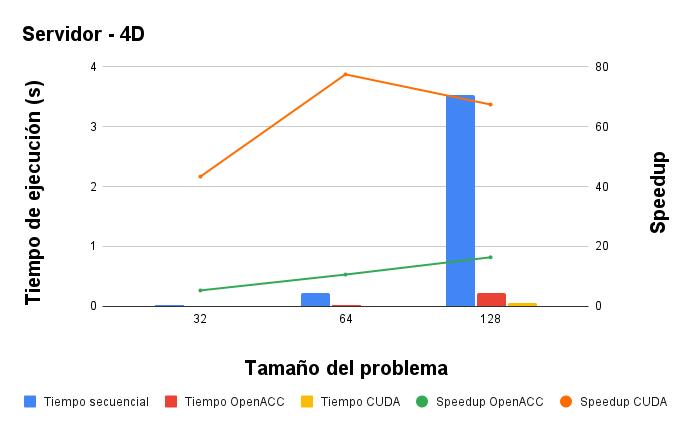
\includegraphics[width=\textwidth]{img/Servidor - 4D.png}
    \caption{Representación gráfica de los tiempos de ejecución y de las aceleraciones obtenidas en el Servidor para la versión 4D }
    \label{GraficoServidor4D}
\end{figure}
\raggedbottom
Hasta ahora, todas los resultados expuestos han sido tomados teniendo en cuenta las transferencias CPU-GPU-CPU, como se comenta en el capítulo \ref{ParalelizacionCUDA}, el uso del paradigma GPGPU requiere que se realicen transferencias de datos desde la CPU a la GPU, y finalmente de GPU a CPU para salvar los resultados (transferencias CPU-GPU-CPU de ahora en adelante). Con el objetivo de demostrar la eficiencia del código desarrollado se deja la Tabla \ref{TiemposServidorTransferencias} donde se muestran los tiempos y aceleraciones obtenidas en el servidor con y sin las transferencias CPU-GPU-CPU.

En la Tabla \ref{TiemposServidorTransferencias} se llegan a obtener una aceleración máxima de 382.23x en la versión 2D y una aceleración de 239.83x en la versión 4D.  
\raggedbottom
\begin{table}[H]
    \centering
    \begin{tabular}{lllllll}
    \multicolumn{1}{c}{} & \multicolumn{1}{c}{} & \multicolumn{5}{c}{CUDA}                                                                                    \\ 
    \cline{3-7}
                         &                      & \multicolumn{2}{l}{Con transferencias CPU-GPU-CPU} &  & \multicolumn{2}{l}{Sin transferencias CPU-GPU-CPU}  \\ 
    \cline{3-4}\cline{6-7}
                         &                      & Min. Time   & Max. Speedup                         &  & Min. Time & Max. Speedup                            \\
    128                  &                      & 0.000172544 & 2.76                                 &  & 0.000178  & 2.68                                    \\
    1024                 &                      & 0.000374784 & 28.69                                &  & 0.000269  & 39.92                                   \\
    4096                 &                      & 0.00271309  & 55.99                                &  & 0.000734  & 207.03                                  \\
    8192                 &                      & 0.0102789   & \textbf{59.31}                       &  & 0.001876  & 324.98                                  \\
    16384                &                      & 0.0450243   & 54.23                                &  & 0.006616  & 369.05                                  \\
    32768                &                      & 0.180257    & 54.22                                &  & 0.025568  & \textbf{382.23}                         \\
                         &                      &             &                                      &  &           &                                         \\
    64                   &                      & 0.00021555  & 13.07                                &  & 0.000172  & 16.42                                   \\
    128                  &                      & 0.00058726  & 38.58                                &  & 0.000301  & 75.27                                   \\
    256                  &                      & 0.00312218  & \textbf{57.73}                       &  & 0.001159  & 155.5                                   \\
    512                  &                      & 0.02524210  & 57.25                                &  & 0.008231  & \textbf{175.57}                         \\
    1024                 &                      & 0.23780300  & 48.59                                &  & 0.095823  & 120.58                                  \\
                         &                      &             &                                      &  &           &                                         \\
    32                   &                      & 0.00032358  & 43.32                                &  & 0.00017   & 82.21                                   \\
    64                   &                      & 0.00284979  & \textbf{77.47}                       &  & 0.000921  & \textbf{239.83}                         \\
    128                  &                      & 0.05238320  & 67.4                                 &  & 0.018837  & 187.43                                  \\
                         &                      &             &                                      &  &           &                                         \\
                         &                      &             &                                      &  &           &                                        
    \end{tabular}
    \caption{Tiempos (en segundos) y aceleraciones obtenidas en el servidor con transferencias CPU-GPU-CPU y sin ellas}
    \label{TiemposServidorTransferencias}
\end{table}



}